\chapter{Introduction}\label{chapter:introduction}
% Introduce Galaxy Interaction, why is it important?
% Remove 'we' from this Introduction. We is only with my own work, not with anyone elses!
In the context of the large scale structure of the \DIFdelbegin \DIFdel{universe}\DIFdelend \DIFaddbegin \DIFadd{Universe}\DIFaddend , galaxies represent a fundamental building block of matter. Their evolution through cosmic time leads to the local \DIFdelbegin \DIFdel{universe }\DIFdelend \DIFaddbegin \DIFadd{Universe }\DIFaddend as we see it today \citep{2005Natur.435..629S}. A key part of its evolution is that of mutual interactions between galaxies. Our best cosmological model, $\Lambda$-Cold Dark Matter, dictates that galaxies assembled hierarchically \citep{1978MNRAS.183..341W, 1991ApJ...379...52W}. Therefore, we must understand the effects of mutual interaction to not just understand galaxy evolution but to better understand our theories of cosmology.

We have come to understand that interaction has multiple impacts on the evolution of galaxies. The first, and most obvious, effect is that it leads to the distortion of the galaxies involved and the formation of distinct tidal features. Early numerical simulations had excellent success recreating, and thus proving, these distortions to the galaxies were from tidal interactions between galaxies \citep{1972ApJ...178..623T}. Thus, tidal features became the primary method by which to identify interacting galaxies.  However, \DIFdelbegin \DIFdel{as our identification methods developed }\DIFdelend it was found \DIFdelbegin \DIFdel{using only visual information led to }\DIFdelend \DIFaddbegin \DIFadd{that datasets identified in this way contained }\DIFaddend high levels of contamination\DIFdelbegin \DIFdel{by close pairs by projection \mbox{%DIFAUXCMD
\citep[e.g][]{2018MNRAS.479..415A, 2020MNRAS.492.2075B, 2022A&A...661A..52P}}\hspace{0pt}%DIFAUXCMD
}\DIFdelend . Often, pairs of systems which appeared interacting or distorted were found to be at very different redshifts; their peculiar morphologies caused by other processes. \DIFaddbegin \DIFadd{These were close pairs by projection rather than physically close together in space \mbox{%DIFAUXCMD
\citep[e.g][]{2018MNRAS.479..415A, 2020MNRAS.492.2075B, 2022A&A...661A..52P}}\hspace{0pt}%DIFAUXCMD
. }\DIFaddend A paramount requirement for the identification of interacting pairs became redshift information, to ascertain \DIFdelbegin \DIFdel{the }\DIFdelend \DIFaddbegin \DIFadd{their }\DIFaddend 3D distances from each other. However, spectroscopic information \DIFdelbegin \DIFdel{across the many million close galaxy pairs we know is limited}\DIFdelend \DIFaddbegin \DIFadd{is not available across many of the millions of close pairs to classify}\DIFaddend .

From the systems we have reliably identified, we have found mutual interaction has further effects on galaxies than morphological disturbance. It is has been found that interaction also causes an increase in the measured star formation \citep{1987ApJ...320...49B, 1992ApJ...400..153M}, higher fractions of active galactic nuclei \citep{2008AJ....135.1877E, 2014MNRAS.441.1297S} and evidence for quenching of the systems involved \citep{1992AJ....104.1039S, 2010MNRAS.407..749G}. This is \DIFdelbegin \DIFdel{particularily }\DIFdelend \DIFaddbegin \DIFadd{particularly }\DIFaddend true of interactions between gas-rich galaxies where the fuel for star formation is readily available and quickly used. Rejuvenation of galaxies can also occur due interactions between gas-rich and gas-poor systems \citep{1992AJ....104.1039S, 2009ApJ...691.1168H}.

The scale, change and impact of these effects is dependent on a host of underlying parameters of the galaxies involved. These include the galactic masses, the orientation of the galaxies and velocity of the encounter. This link between these parameters and the characteristics of the final system have been poorly explored. In this work, we \DIFdelbegin \DIFdel{will investigate this relationship by exploring }\DIFdelend \DIFaddbegin \DIFadd{create }\DIFaddend a large sample of interacting galaxies \DIFdelbegin \DIFdel{that we create and }\DIFdelend \DIFaddbegin \DIFadd{using a new machine learning algorithm - }\texttt{\DIFadd{Zoobot}} \DIFadd{- and use it to investigate this relationship. We then }\DIFaddend describe a new software to extract their underlying \DIFdelbegin \DIFdel{parmeters}\DIFdelend \DIFaddbegin \DIFadd{parameters for further study}\DIFaddend . For now, however, it would be prudent to begin this discussion by exploring the definition of a galaxy, and outline the major work already conducted into linking galaxy interaction to its underlying parameters and, furthermore, with galaxy evolution.

\section{What is a Galaxy?}
% Give a simplified idea of a galaxy.
% Basic building blocks of a galaxy.
% But only a simplified example!
\noindent For the purposes of this work, a galaxy will be the smallest unit of mass we will consider. A galaxy is a gravitationally bound system of gas, dust, stars and dark matter. The orbits and kinematics of each of these components leads us to different classifications of galaxies. \DIFdelbegin \DIFdel{The orbits of these components is often about }\DIFdelend \DIFaddbegin \DIFadd{At the galactic centre, there is often }\DIFaddend a supermassive blackhole (SMBH)\DIFdelbegin \DIFdel{at the galactic centre}\DIFdelend . While almost all examples of galaxies have a SMBH at their centre, there are some examples where it is speculated they do not \citep{2001AJ....122.2469G}. If the stars, gas and dust \DIFdelbegin \DIFdel{about this SMBH have been orbiting }\DIFdelend \DIFaddbegin \DIFadd{orbiting the galactic centre of mass have been }\DIFaddend unperturbed for a long period of time they flatten into a disk. The disk is split into a thick and thin component. Their general sizes are dictated by the history of the galaxy, and whether they have interacted or merged with many other galaxies in their history. Such harassment by other galaxies leads to heating of this disk. This heating takes the form of increased peculiar motion in the stellar orbits. This heating contributes not only to the thick disk, but can also lead to the growth of a bulge component in the galaxy \citep{2010ApJ...715..202H, 2017ApJ...837L...8B}. The bulge can be grown by other, secular, processes but we will focus on interaction and merging.

The bulge component is composed of stars whose orbit has been heated by changes in the gravitational potential due to galaxy interaction and harassment. This leads to new orbits that form a spherical bulge component around the galactic centre. This leads the galaxy to have a bulge and disk component, with the bulge composed of a spherical component of stars while the disk is formed of stars and gas continuing in unperturbed orbits. This is the simple view of a classic disk galaxy. Many disk galaxies do not show bulges at all, or show a pseudobulge \citep{2009MNRAS.399..621G}. This remains, at least partially, dependent on the merger history of the galaxy. If a galactic interaction leads to a strong enough merger the entire galactic disk is heated and can be destroyed. This leads to a completely spheroidal galaxy called an elliptical galaxy \citep{1977egsp.conf..401T, 2006MNRAS.366..499D}. Between these two galaxy types - disk and elliptical - lie lenticular galaxies. These are systems that have used most of their gas across their disk and are beginning to exhibit the same features as elliptical galaxies. Whether this is due to mergers \citep{2004ApJ...616..192C, 2005ApJ...621..246B} or via environmental and secular effects \citep{2002MNRAS.330..251M, 2018MNRAS.476.2137R} remains debated. What this demonstrates, however, is the stellar dynamics of galaxies is complex and determined according to the assembly history of each.

The stars, gas and dust are embedded in a much larger, spherical halo. This galactic halo has two different matter components: baryonic and non-baryonic. The baryonic component is formed of very diffuse, ancient stars that form the stellar halo, stellar streams or globular clusters which orbit around the galaxy. The non-baryonic component is formed of dark matter. What dark matter is precisely is still debated, but this spherical dark matter halo extents out to many times the luminous matter of the galaxy. In general, all examples of galaxies are embedded in a dark matter halo \cite[although there are some debated exceptions as described in][]{2018Natur.555..629V}. This dark matter halo has also been imperative to our understanding of how galaxies form, evolve and interact.

For much of the history of extragalactic astrophysics, the idea that galaxies could interact and merge was thought to be very improbable except in dense clusters. The small radii (and, therefore, cross section) of the luminous matter in galaxies led astronomers to believe that the probability of an interaction was close to 0 and that galaxies were island universes \DIFdelbegin \DIFdel{\mbox{%DIFAUXCMD
\citep{1926ApJ....64..321H}}\hspace{0pt}%DIFAUXCMD
}\DIFdelend \DIFaddbegin \DIFadd{\mbox{%DIFAUXCMD
\citep{1755anth.book.....K, 1917PASP...29..206C}}\hspace{0pt}%DIFAUXCMD
}\DIFaddend . However, with the development of the idea of the dark matter halo, it was realised that the probability of galactic systems interacting in the field was reasonable. Over time the idea that galaxy interaction and merging would have a significant impact on galaxy evolution was developed. \DIFdelbegin \DIFdel{In fact, the merger rates of galaxies }\DIFdelend \DIFaddbegin \DIFadd{Today, merger rates }\DIFaddend through cosmic time is a well studied concept \DIFaddbegin \DIFadd{and test }\DIFaddend of our cosmological models\DIFdelbegin \DIFdel{with observations and simulations}\DIFdelend .

\section{Galaxy Assembly Across Cosmological Time}
\noindent Galaxies throughout cosmic history have been assembling and accreting matter. Studies at high redshifts reveal that galaxy structure is significantly different compared to the local volume. Initially, galaxies were very small systems that formed from gravitational instability \DIFdelbegin \DIFdel{thoughout }\DIFdelend \DIFaddbegin \DIFadd{throughout }\DIFaddend the early cosmos \citep{1993MNRAS.262..627L}. These instabilities were generated by the physical processes of the very early Universe brought about by its small scale. From these initial density perturbations arose small systems which accreted from the surrounding gas\DIFdelbegin \DIFdel{and dust. These early galactic systems were much smaller than those we see today. These }\DIFdelend \DIFaddbegin \DIFadd{. These }\DIFaddend galaxies had peculiar morphologies \citep{2005ApJ...627..632E} with disk galaxies beginning to dominate at $z\approx3 - 6$ \citep{2022ApJ...938L...2F}. These early systems formed stars at a much higher rate than the present day. While these systems were accreting much of their matter to gain mass, the Universe was expanding. At this time the rate of galaxies interacting and merging was also greater than today \citep{2010ApJ...715..202H, 2011ApJ...742..103L}, reaching as high as 50\% at $z\approx6$ \citep{2009MNRAS.397..208C, 2009MNRAS.394L..51B}. This provided a peak in the cosmic star formation \DIFdelbegin \DIFdel{of the }\DIFdelend history through $1 < z < 3$ where approximately half of all stellar mass was formed \citep{2005ApJ...625..621B}.

\DIFaddbegin \DIFadd{However, it is not clear that the only driver of this higher star formation rate in the early universe was mergers. More recent works have shown that secular processes may have also played a significant role. It has been noted that the fraction of clumpy galaxies was significantly higher at these times \mbox{%DIFAUXCMD
\citep{2012ApJ...760..130S, 2020MNRAS.499.5241C,  2023ApJ...955...92V}}\hspace{0pt}%DIFAUXCMD
. Clumps within galaxies are large, star forming regions which form due to violent disk instabilities. The size, and longevity of the clumpy region is found to correlate closely to the gas fraction of the galaxy it is in \mbox{%DIFAUXCMD
\citep{2021MNRAS.505.3579F}}\hspace{0pt}%DIFAUXCMD
. This points to disc galaxies in the early Universe containing much higher gas fractions \mbox{%DIFAUXCMD
\citep{2010Natur.463..781T, 2023ApJ...943...82S} }\hspace{0pt}%DIFAUXCMD
than their local counterparts. Therefore, not only was the merger fraction higher at earlier epochs, but the internal properties of galaxies differed and were much more extreme.
}

\DIFadd{However, as stated, the merger rate was also changing throughout this epoch of the Universe. }\DIFaddend Figure \ref{fig:merger-rate} shows the changing merger rate through cosmic time. As \DIFaddbegin \DIFadd{shown, }\DIFaddend the merger rate \DIFdelbegin \DIFdel{increased, peaked and then declined, it }\DIFdelend \DIFaddbegin \DIFadd{has been decreasing with redshift, while the internal environment of galaxies has become less extreme, which has }\DIFaddend had profound effects on both the star formation density of the Universe and the morphology of those galaxies within it. From $z = 1$, the once massive galaxies with rapid star formation have transformed into bulge-dominated galaxies \DIFdelbegin \DIFdel{containing SMBHs }\DIFdelend \citep{2007ApJ...654..858B}. At lower redshifts we find that the majority of the stellar mass is contained within bulge dominated systems. These galaxies are dominated by old stellar components and have little ongoing star formation \citep{2002AJ....124..646H, 2004ApJ...608..752B}.
\DIFdelbegin \DIFdel{Thus, showing that mergers played a significant role in star formation of the past. 
}\DIFdelend 

\begin{figure}
\centering
\includegraphics[width=0.95\textwidth]{Introduction/figures/merger-rates.png}
\caption[The declining merger rates from z = 3 to z = 0.]{The clearly declining merger rates from $z = 3$ to $z = 0$. This is Figure 3 of \citet{2010ApJ...715..202H}. This study looked at the history of a simulated set of galaxies of various stellar mass, and investigated the decrease in the merger fraction as a function of redshift and baryonic mass. As shown, for all mass bins and methods of identifying mergers (the different lines) the merger rate decreases. This is only not true for mergers between very high mass systems and low mass systems (in the bottom right of this plot). Thus, mergers between high and low mass systems may still have some driving force in the cosmic star formation rate density.}
\label{fig:merger-rate}
\end{figure}

This gives us an avenue by which to link observed galaxy morphologies to their merger histories. We split them into two distinct populations. One is of galaxies with an intense merger history, leading to the complete destruction of their disks and their domination by older stellar populations. The other is of those with a relatively \DIFdelbegin \DIFdel{relaxed }\DIFdelend \DIFaddbegin \DIFadd{non-violent }\DIFaddend merger history. These non-destructive interactions and mergers served to feed the gas within the galactic disks and increase their mass, while maintaining their star formation rates. These systems are dominated by younger stellar populations, with star formation continuing to the present epoch. Thus, starting from the observations of morphology, we can make assumptions about the internal gas content, star formation and, therefore, colour of galaxies.

\section{Galaxy Morphology \& Galactic Properties}\label{galaxy-morphology}
\noindent Galaxy morphology, and its change with time, is the study and measure of a \DIFdelbegin \DIFdel{galaxys'}\DIFdelend \DIFaddbegin \DIFadd{galaxy's }\DIFaddend shape and features. A striking distinction in galaxy morphology is between disk and elliptical galaxies, the primary breakdown in the famous `Hubble tuning fork' shown in Figure \ref{fig:hubble-tuning} \citep{1936rene.book.....H}. This \DIFdelbegin \DIFdel{was thought to be a map of galaxy evolution with }\DIFdelend \DIFaddbegin \DIFadd{mapped the complexity of galaxy morphology, with simple }\DIFaddend early-type elliptical galaxies on the left \DIFdelbegin \DIFdel{which would evolve to the }\DIFdelend \DIFaddbegin \DIFadd{and complex }\DIFaddend late-type disk and spiral galaxies on the right. \DIFdelbegin \DIFdel{However, this was found not to be the case with early-type elliptical galaxies being older than late-type disk galaxies. So, while this classification scheme was not a direct evolutionary pathway it was found to be indicative of the merger history of a galaxy. }\DIFdelend Elliptical galaxies are spheroidal systems, with high internal velocity dispersions. Such systems are often created as the result of mergers and cannibalism of smaller systems to interactions with counterparts of a similar mass \citep{1996MNRAS.283.1361B, 2006MNRAS.366..499D}. Disk galaxies, on the other hand, are rotationally-dominated systems with a central bulge whose size is crucially dependent on the merger history \citep{1992ApJ...393..484B, 2010ApJ...715..202H, 2017ApJ...837L...8B}. In fact, galaxies that appear to have no bulge component at all likely have had no merger event in the last few Gyrs \citep{2012ApJ...756...26M}.

\begin{figure}
\centering
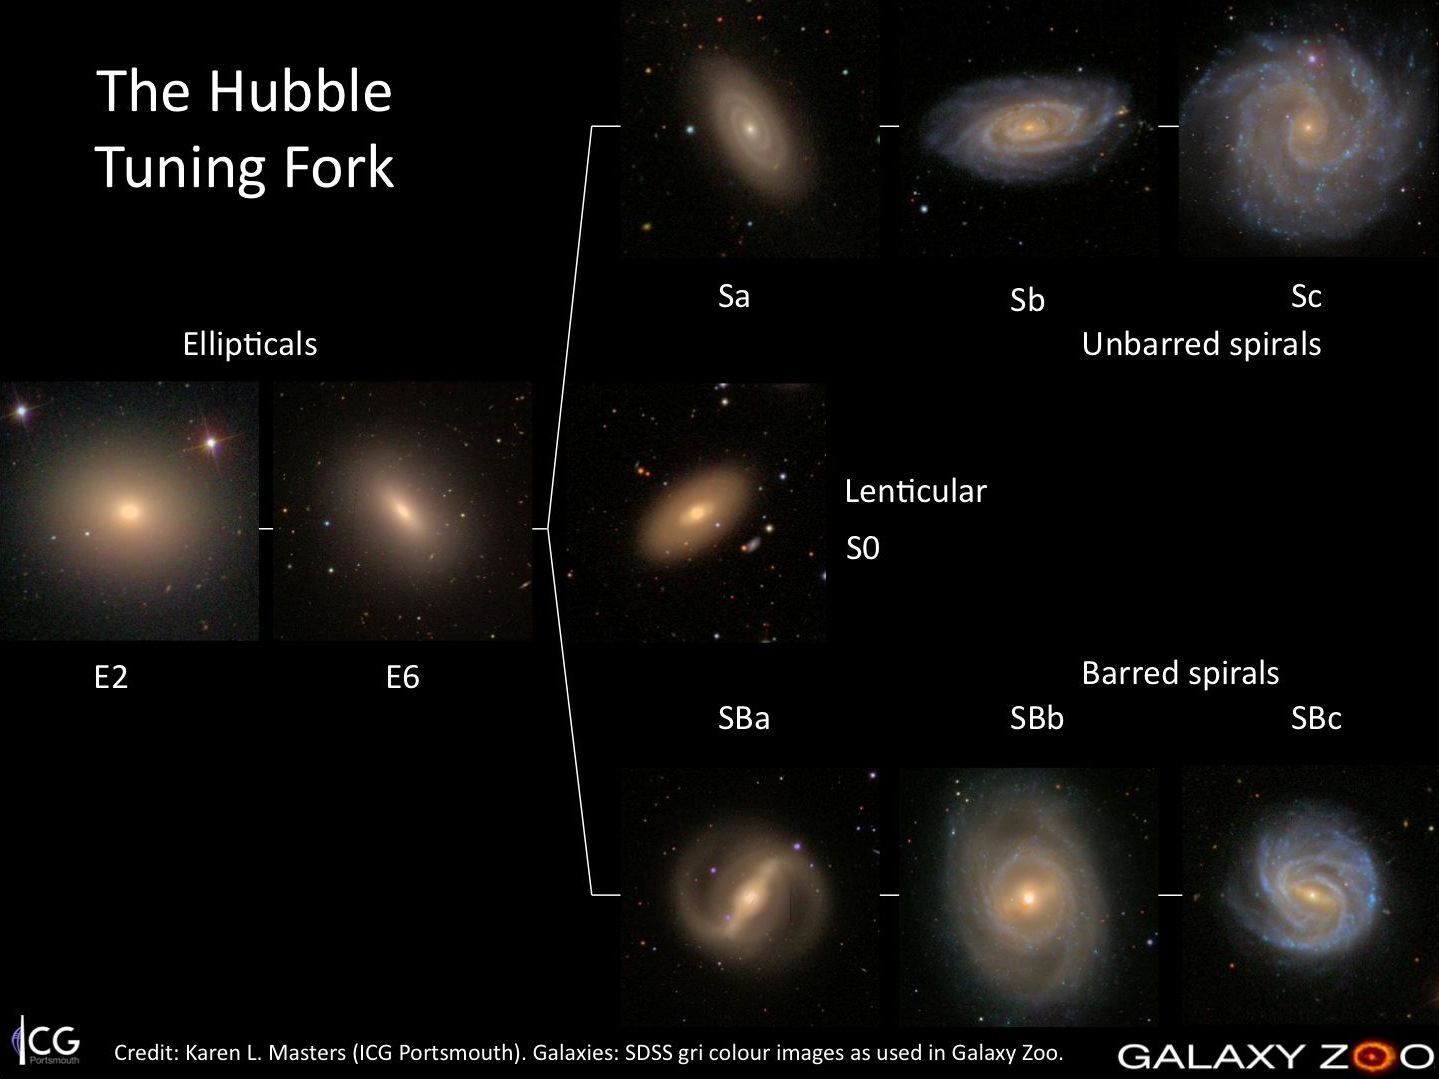
\includegraphics[width=0.95\textwidth]{Introduction/figures/hubble-tuning-fork.jpg}
\caption[The Hubble tuning fork.]{The Hubble tuning fork. Credit goes to the Galaxy Zoo collaboration (and specifically Karen Masters) for the creation of this figure. \DIFdelbeginFL \DIFdelFL{What was once thought of as an evolutionary track for galaxies, is now a widely adopted classification system for them based on morphology. }\DIFdelendFL On the left, we have elliptical systems - so called early-type galaxies - which are often `red and dead' systems. They have an intense merger history, which has destroyed their disk component and caused them to use the majority of their gas in star formation. On the right, we have two different kinds of disk galaxies. Ignoring the bar or un-barred part of this, they are systems which have a less intense merger history and have only accreted smaller systems into them. This serves to enhance their gas disk, and preserve their disk component.}
\label{fig:hubble-tuning}
\end{figure}

This is also reflected in the observed colour of disk and elliptical galaxies. Observational colours in this context are the comparison of flux in two different wavelength ranges: one capturing the flux of young, star forming regions while the other captures the flux from old, low mass stars. In combination, these young and old stars, constitute a stellar population. Stellar populations have well defined spectral energy distributions (SEDs) based on their age and, indirectly, to a galaxys' star formation rate (SFR) and gas mass. When star formation is occurring rapidly, and the SFR is very high, lots of young, luminous OB-type stars form. The flux from these stars falls mainly in our blue filters, in the rest wavelength of ultraviolet. These stars have lifetimes of only a few million years and, therefore, die very quickly. Thus, if stars are forming slowly, and the SFR is very low, these OB-type stars will die and not be replaced. This leaves an older stellar population, mainly composed of G- to M-type stars which lie primarily in our green and red filters, with wavelengths in the optical. 
\DIFaddbegin 

\DIFadd{A secondary method to measure the time since active star formation is by using the $4000\textrm{\AA}$ break \mbox{%DIFAUXCMD
\citep{1998ApJ...504L..75B}}\hspace{0pt}%DIFAUXCMD
. This is a large step in an observed galaxies spectra at around $4000\textrm{\AA}$ caused by the absorption of high energy radiation from metals in stellar atmospheres. These metals are formed in high luminosity stars and then injected into the population via supernovae. So, the higher metallicity (and older) a stellar population is, the larger the $4000\textrm{\AA}$ break will be and the longer it will have been since active star formation and the redder the population. }\DIFaddend Thus, the SFR and age of the dominant stellar population of a galaxy influences their observed colour.

The SFR, then, is highly dependent on the gas mass present in the galaxy. This gas must be \DIFaddbegin \DIFadd{cold, }\DIFaddend molecular gas, with little energy so it is able to form massive clouds that fragment and undergo collapse \citep{1965MNRAS.130...97G, 1972ApJ...176L...9Q}. From models of individual clouds, it was noted that the \DIFaddbegin \DIFadd{cold }\DIFaddend gas density was related to the density of star formation in galaxies \citep{1959ApJ...129..243S}. This was further refined to be a global law in disk galaxies in particular in \citet{1998ApJ...498..541K}. In this, it was shown that the surface area of star formation is directly related to the surface area of \DIFaddbegin \DIFadd{cold }\DIFaddend gas by 

\begin{equation}\label{eq:ks-law}
\Sigma_{SFR} \propto \Sigma_{Gas}^{n}. 
\end{equation}

\noindent This relation has been found to be $n\approx1.3$. Thus, two things are happening here, if a galaxy has \DIFaddbegin \DIFadd{cold }\DIFaddend gas, it has star formation and if it has star formation \DIFaddbegin \DIFadd{with little dust}\DIFaddend , it will be observed to be blue and vice versa.

When observing populations of red galaxies, those dominated by older stellar populations, it has been found they are often elliptical galaxies \citep{1992MNRAS.254..589B}. These galaxies have a more violent merger history that has destroyed the ordered rotationally dominated component of a galactic disk and, in the process, either removed or used the gas within the galaxy \citep{1976ApJ...204..365F}. As a result of this, the current gas mass and density are very low which leads to the SFR being also low.

% Talk about the blue-ness of disk galaxies.
The opposite is true for disk galaxies. As stated previously, these systems have had a less \DIFdelbegin \DIFdel{tumultous }\DIFdelend \DIFaddbegin \DIFadd{tumultuous }\DIFaddend merger history - \DIFdelbegin \DIFdel{particularily }\DIFdelend \DIFaddbegin \DIFadd{particularly }\DIFaddend since $z \approx 1$. An indicator of the merger or interaction history in disk galaxies is the size and shape of the bulge component \citep{2011MNRAS.414..888E}. However, because of the plentiful gas, dust and ordered rotation in the galactic disk the SFR within is larger than elliptical galaxies. The surface density of gas within the disk is much larger than in elliptical galaxies providing the ideal for star formation. Spiral arms can exist in such galaxies, containing large filaments of gas and dust. They contain areas where large molecular clouds can \DIFdelbegin \DIFdel{condence}\DIFdelend \DIFaddbegin \DIFadd{condense}\DIFaddend , fragment and then collapse into new stars. These star forming regions will be young enough that massive OB-type stars will form, which in turn changes the underlying SED of the galaxy that we observe. The blue filter will contain more flux, and therefore, the galaxy appears blue when comparing the red and blue filters.

\begin{figure}
\centering
\includegraphics[width=0.95\textwidth]{Introduction/figures/population-distribution.png}
\caption[The distribution of galaxies in colour-colour space showing two distinct populations in a clear bi-modal structure.]{The distribution of galaxies in colour-colour space showing two distinct populations in a clear bi-modal structure. This is using the u-band and r-band filters and, therefore, the closer to 0 on the y-axis the bluer the galaxy. Left plot: the top population is the blue cloud, primarily composed of disk galaxies with young, star forming stellar populations. The bottom population is the red sequence, primarily composed of more massive elliptical galaxies which are gas poor and quiescent. Between these two populations lies the green valley, marked by the green lines. This is believed to be a transitional population moving between the blue cloud and red sequence for debatable reasons. To further show the split with morphology, the panels on the right split the colour-mass space into early-type (elliptical) galaxies and late-type (disk) galaxies. Note, this is Figure 2 of \citet{2014MNRAS.440..889S}}
\label{fig:blue-red-population}
\end{figure}

% Now, talk about the blue and red sequence.
This gives rise to two distinct populations of galaxies: old, red elliptical galaxies and young, blue disk galaxies. When plotting colour-colour or colour-magnitude diagrams, there is clear bi-modality which separates these two populations with the `green valley' running between them \citep{2001AJ....122.1861S}. Figure \ref{fig:blue-red-population} shows the colour-colour distribution if the two populations. In this Figure, we clearly can see the blue population - blue cloud - and the red population - red \DIFdelbegin \DIFdel{sequance }\DIFdelend \DIFaddbegin \DIFadd{sequence }\DIFaddend - beneath it with the green valley in between. The green valley is a disputed area of this distribution. Some works claim that it is a rapid transition phase \citep{2007ApJS..173..315S, 2015MNRAS.450..435S}, where galaxies are moving between the two populations due to different processes. Others, meanwhile, show that the picture is much more complicated, with morphology and environment playing an important role that dictates the decline in star formation \citep{2014MNRAS.440..889S}. However, \DIFdelbegin \DIFdel{what is definitive is }\DIFdelend the rule elliptical galaxies are always red and disk galaxies are always blue is not \DIFdelbegin \DIFdel{ubiquitous }\DIFdelend \DIFaddbegin \DIFadd{universally true }\DIFaddend \citep{2022MNRAS.510.4126S}. Examples of blue ellipticals and red spirals do exist \citep{2009MNRAS.396..818S, 2010MNRAS.405..783M, 2022AJ....163..150K} and they are the subject of intense debate and study in the current field. However, as a general guideline for the expected properties of a galaxy the colour and morphology are deeply interdependent on one another.

% Want to introduce the idea of starburst galaxies, remnants and such here.
There are also many types of systems that do not fit this simple morphological definition of galaxies. Starburst galaxies are often very morphologically irregular and have measured SFRs far in excess of expectation for their mass. These then lead into post-starburst galaxies and merger remnants, who are the complete opposite and have measured very low SFRs. \DIFdelbegin \DIFdel{These are often called quiescent galaxies. These highly irregular systems have direct interplay, however, with their }\DIFdelend \DIFaddbegin \DIFadd{Thus, a parameter such as the SFR of the system is highly dependent on its }\DIFaddend merger histories and\DIFaddbegin \DIFadd{, as we will find, its }\DIFaddend surrounding environments \citep{2018MNRAS.477.1708P, 2020MNRAS.493.3716H}. In fact, it has been found that in cluster environments, the fraction of disk galaxies drops to $\leq$10\% when compared to $\approx$60\% in the field.

The effect of the galactic environment on a galaxy should also not be understated. There are many ways to define the galactic environment, but it is most commonly associated with the number density of galaxies about them \citep{2003ApJ...585..694E, 2004ApJ...615L.101B}. There are three broad classifications of environment: field, filament and cluster. A field galaxy is one with neighbours, and is in relative isolation. A filament galaxy has some neighbours, but their influence is minimal. A cluster galaxy is one in which a large number of other galaxies are bound in large galactic super-structures. In such an environment, SFRs are suppressed \citep{2006MNRAS.373..469B} by ram pressure stripping and \DIFdelbegin \DIFdel{galaxy morphology is highly irregular }\DIFdelend \DIFaddbegin \DIFadd{the dominant morphologies are elliptical and irregular galaxies }\DIFaddend due to constant interaction and \DIFdelbegin \DIFdel{merging. In these }\DIFdelend \DIFaddbegin \DIFadd{harassment. In such }\DIFaddend environments, the relation between galaxy morphology and the underlying processes is almost completely broken by interference from the environment.

\DIFdelbegin \DIFdel{Thus, galaxies }\DIFdelend \DIFaddbegin \DIFadd{Galaxies }\DIFaddend in the field or in filaments are of particular interest. Here, we can study the direct link between morphology and the underlying processes of galaxies. And these, in turn, are highly dependent on galaxies underlying merger and interaction histories. So, what is this relation? As stated previously, the influence of interaction and merging accelerates the evolution of rotational systems to dispersion dominated systems. However, there are many more subtle \DIFdelbegin \DIFdel{affects }\DIFdelend \DIFaddbegin \DIFadd{effects }\DIFaddend that can be attributed to galactic merging and interaction. For instance, \DIFdelbegin \DIFdel{if }\DIFdelend two galaxies can be brought into a state of starbursting due to merging \citep{2008MNRAS.385L..38M}. This completely changes the \DIFdelbegin \DIFdel{underlying }\DIFdelend SED of the \DIFdelbegin \DIFdel{galaxies involved}\DIFdelend \DIFaddbegin \DIFadd{galaxy}\DIFaddend , and can lead to the rapid quenching both systems \citep{2018MNRAS.476.2591V, 2022MNRAS.517L..92E}. Depending on when we observe such a galaxy, we can find either a much bluer or redder galaxy than expected \citep{2007A&A...468...61D}. However, these effects are also debated, with some studies finding that galaxy interaction does not induce significant change in the SFR, and therefore, the underlying SED of the galaxy population \citep{2003A&A...405...31B}. So, why is this? It transpires that the effects of a galaxy merger or galaxy interaction is dependent on the underlying parameters of the galaxies themselves. This leads to multiple classifications of galaxy interactions which each lead to different outcomes for the galaxies involved. 

\section{Categorisation of Mergers}
\noindent The effects of galaxy interaction and merging is dependent on multiple factors and underlying parameters. A key parameter to the destruction or survival of a disk is the mass ratio between the two systems \citep{2005A&A...437...69B, 2008MNRAS.384..386C}. The impact parameter also has significant influence over the final morphology over the system, however, we will discuss this further in \DIFdelbegin \DIFdel{Chapter }\DIFdelend \DIFaddbegin \DIFadd{Section }\DIFaddend \ref{sec:int_effects}. The gas content of each galaxy also has an effect on the changes of the internal SFR of the systems. The large change in the systems we see based on these parameters gives rise to many different categorisations of galaxies. For the mass ratio, we define a major, a minor and a micro interaction. These are the ratios of the primary galaxy mass (the more massive galaxy) and the secondary galaxy mass (the less massive galaxy). 

These are then further sub-divided into two \DIFdelbegin \DIFdel{seperate }\DIFdelend \DIFaddbegin \DIFadd{separate }\DIFaddend categories based on their gas content: a wet merger or a dry merger. This refers to the gas mass and colour of both galaxies. A wet merger involves \DIFdelbegin \DIFdel{lots of gas in the two galaxies colliding}\DIFdelend \DIFaddbegin \DIFadd{galaxies which have a high gas fraction}\DIFaddend , and therefore, lots of resultant star formation. Both of the involved galaxies are \DIFdelbegin \DIFdel{blue, and }\DIFdelend often disk-dominated galaxies. A dry merger involves little gas, and is often the merger of massive, red elliptical galaxies. There are also intermediate categorisations based on the amount of gas, such as damp mergers (where there is some gas, but not enough to dramatically increase star formation) and mixed mergers (mergers between gas-poor and gas-rich systems), however, we will focus on the binary definition of wet and dry mergers.

% Change the intro sentence below to introduce new classification we're discussing.
Depending on the classification\DIFdelbegin \DIFdel{of }\DIFdelend \DIFaddbegin \DIFadd{, }\DIFaddend an interaction leads to specific outcomes for the interacting galaxy system. A major interaction is when the galaxies involved have a mass ratio of approximately 1:1. Some definitions vary, however, and allow this limit to go down to 1:3. For the purposes of this work, they must have a mass ratio of at least 1:3. Major interactions are the most devastating to the morphology of the systems involved, with the forces upon them causing severe morphological distortion and the formation of tidal features (described further in the following Chapter). If the two systems merge, there is complete destruction of the disks in both galaxies and the post-merger remnant will be highly irregular. If this is also a wet merger \DIFdelbegin \DIFdel{one }\DIFdelend we would also expect a significant increase in the SFRs of both galaxies \citep{1994ApJ...425L..13M, 1996ApJ...464..641M, 2006AJ....132..197W}. We also find that wet major mergers have an increased AGN fraction, which suggests that such a merger may play a role in starting nuclear activity \citep{2007MNRAS.375.1017A, 2011MNRAS.418.2043E, 2012ApJ...746L..22K}. The opposite of this is true when a major interaction is dry, where only a small increase in SFR is found in the nuclear region of the galaxies \citep{2004ApJ...614..586S, 2006ApJ...640..241B}.

A minor interaction has less catastrophic consequences for the morphology of one of the two galaxies. This is defined as an interaction where the mass ratio is less than 1:3 but greater than 1:10. Due to this large mass disparity, the morphology of the primary galaxy is relatively unaffected by such an interaction. However, the secondary galaxy will be almost completely destroyed by the encounter. If only an interaction occurs, the secondary will be \DIFdelbegin \DIFdel{higly }\DIFdelend \DIFaddbegin \DIFadd{highly }\DIFaddend disrupted forming a long and stretched tidal tail as it moves through the orbit. When these systems merge, we observe small increases in the SFR of the primary. There is ongoing work investigating whether such mergers were actually a primary driver of star formation in galaxies across cosmic time through rejuvenation of gas \DIFdelbegin \DIFdel{resevoirs }\DIFdelend \DIFaddbegin \DIFadd{reservoirs }\DIFaddend within the primary galaxy \citep{2007A&A...476.1179B, 2014MNRAS.440.2944K, 2022MNRAS.511..607J}. Finally, a micro interaction is one in which the mass ratio between the primary and secondary galaxies is less than 1:10. This sees the complete destruction of the secondary galaxy, whether a flyby or a complete merger. These can form stellar streams about their primary galaxy and are often absorbed by the primary with very little change in its morphology.

\begin{figure}
\centering
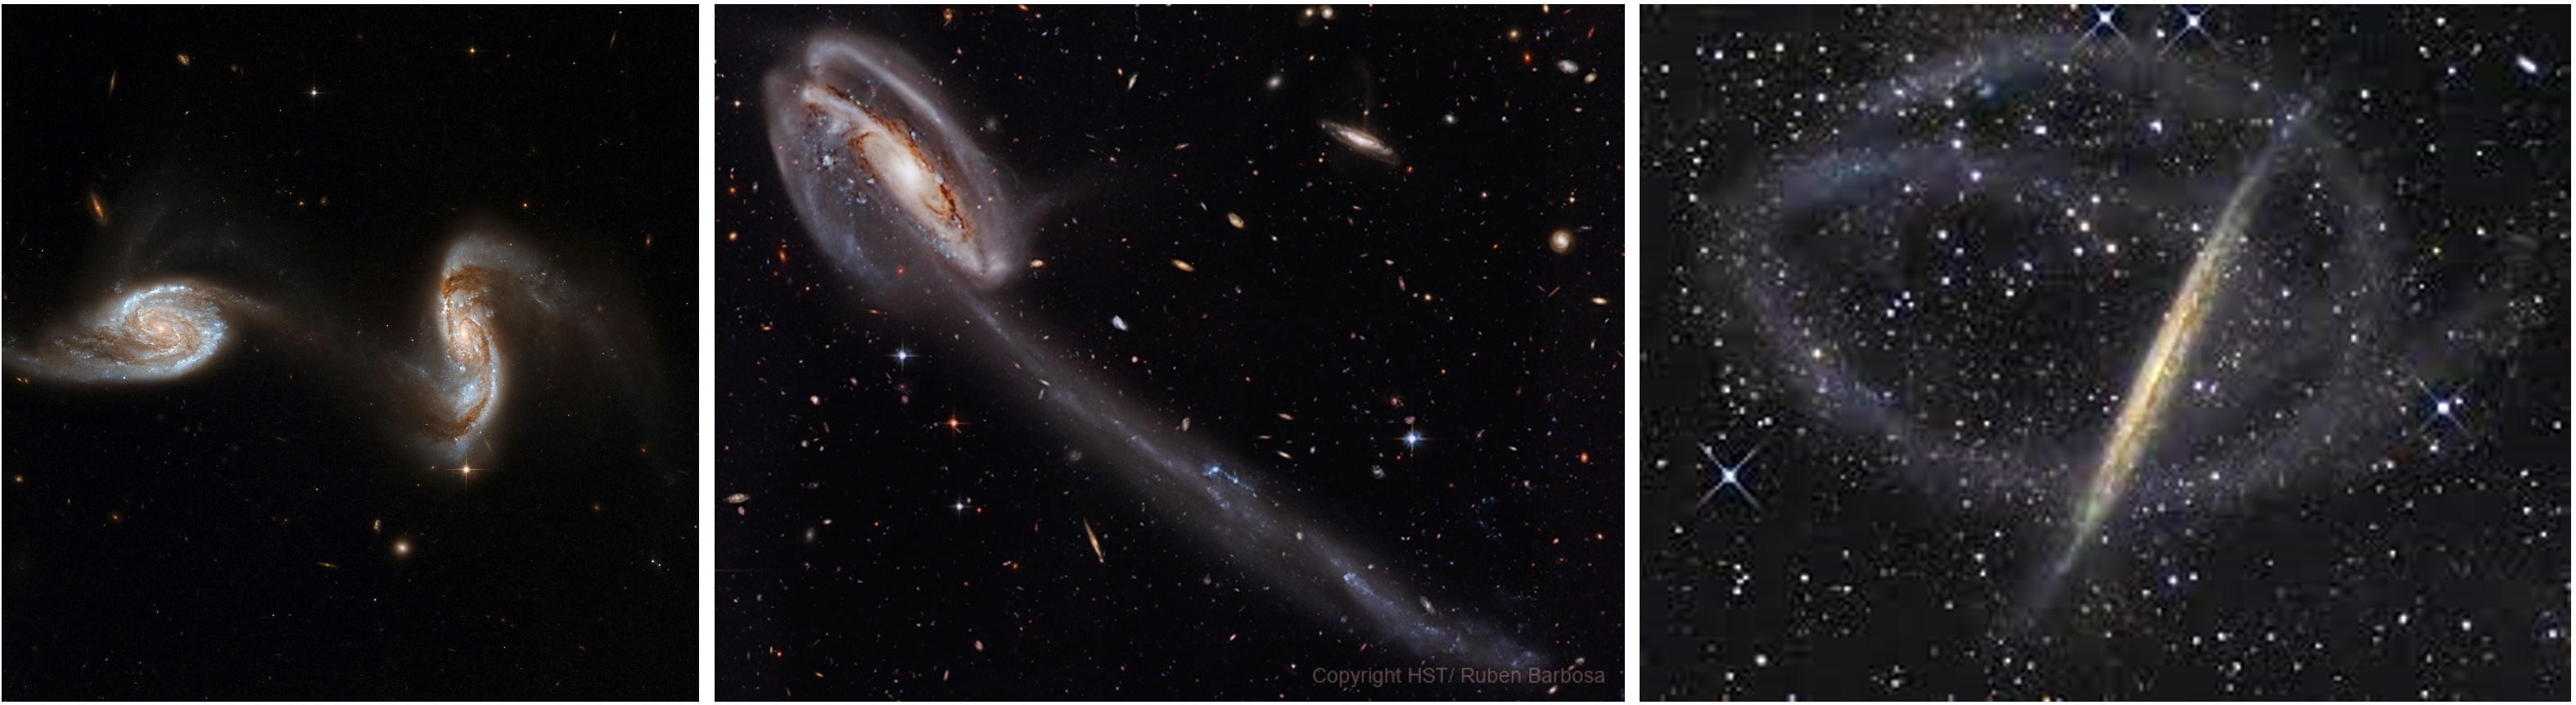
\includegraphics[width=0.95\textwidth]{Introduction/figures/combined-examples-mergers.jpg}
\caption[Examples of a major, a minor and a micro interaction.]{Examples of a major, a minor and a micro interaction. Each of these are wet interactions, containing lots of gas and therefore, increases the rate of formation of stars. These are the Arp 240, Arp 188 and NGC 5907 systems, respectively. Here, we show the famous double looped stellar stream of NGC 5907 but point out that the existence of the second loop is in dispute and that we only show it here for illustrative purposes \citep{2019ApJ...883L..32V}. From major to micro interactions, we see decreasing impact and change in the morphology of the primary galaxies but always the complete destruction of the secondary.}
\label{fig:merger-clsfs}
\end{figure}

Figure \ref{fig:merger-clsfs} displays examples of each of the different merger categories we have defined here. These, from left to right, are the Arp 240, Arp 188 and NGC 5907 systems. They each show a major, minor and micro interaction, respectively, and demonstrate the change in effect the mass ratio has on the morphology of the galaxies involved\DIFdelbegin \DIFdel{. From }\DIFdelend \DIFaddbegin \DIFadd{, from }\DIFaddend Arp 240, with the complete distortion of the galactic disks and formation of tidal features to NGC 5907 where the primary galaxy is barely disturbed at all. Thus, the different categories of interactions and mergers have very different impacts on the systems involved. We will now discuss, in depth, the effects that interaction has on these galaxies and specifically explore the formation of morphological disturbances like tidal features, changes in the SFR and the increase in AGN fraction.

\section{Effects of Galaxy Interaction}\label{sec:int_effects}
% Here, present examples of interacting galaxies and the context in which we're talking about them.
Until the work of \citet{1972ApJ...178..623T}, the \DIFdelbegin \DIFdel{idea }\DIFdelend \DIFaddbegin \DIFadd{probability }\DIFaddend that two galaxies would encounter each other and interact was thought to be \DIFdelbegin \DIFdel{minute}\DIFdelend \DIFaddbegin \DIFadd{negligible}\DIFaddend . We now understand that galaxy interaction plays an important, and fundamental role in the evolution of galaxies. As stated previously, they have multiple effects upon the systems undergoing the interaction. The specific effects of interaction rests on a host of parameters. We have discussed the mass ratio and gas content and mentioned the impact parameter but there is also the orientation of the interaction, the relative sizes of the galaxies and the point in the dynamical history of the interaction we are observing. Thus, in this Chapter, we will explore how these different underlying parameters link to the physical processes we observe in interacting and merging galaxies.

% For each of these sections below, I want to do a deep dive on how each process is driven. Will maybe mention simulations throughout, but we shall see?
\subsection{Morphological Distortion: Tidal Features}
% Introduce the gravitational potential in this paragraph.
\noindent As previously discussed, galaxies are large gravitationally bound systems of stars, gas, dust and dark matter. Upon a close encounter between two galactic systems, these components experience strong gravitational forces which disrupt their ordered layout. As the galaxies move through their relative orbits, the gravitational potential changes at an accelerating rate. This imparts energy into the ordered components of the galaxies, and causes thermalization of their internal motions. This leads to violent relaxation, where the stellar orbits are so altered they no longer follow their prior orbits. However, the energy in the system must be conserved. Thus, as the internal stellar motions within the galaxy thermalizes, the energy in the \DIFdelbegin \DIFdel{galaxy's }\DIFdelend \DIFaddbegin \DIFadd{galaxies }\DIFaddend orbits decay via dynamical friction. If this decay is large enough, the energy in the \DIFdelbegin \DIFdel{galaxy's }\DIFdelend \DIFaddbegin \DIFadd{galaxies }\DIFaddend orbit may be sufficiently reduced to no longer escape from one another and they will eventually coalesce to leave a single merger remnant. 

The changing \DIFdelbegin \DIFdel{graviational }\DIFdelend \DIFaddbegin \DIFadd{gravitational }\DIFaddend fields as the two galaxies encounter each other leads to radial distortion of each galaxy. If stellar material, including gas, dust and stars, is close to the edge of the galaxy a combination of the galactic rotation and radial elongation lead to it being sheared off and away from the galaxy. This forms two `tidal tails` in the system, one leading and one \DIFdelbegin \DIFdel{proceding }\DIFdelend \DIFaddbegin \DIFadd{proceeding }\DIFaddend the motion of the galaxy. Dependent on the geometry of the encounter, the trailing tail of one galaxy and the preceding tail of the other can form a `tidal bridge' - a linking of the two systems. An example of both of these is the interacting pair Arp 240, shown in left hand plot of Figure \ref{fig:merger-clsfs}. 

The geometry of the bulk motion of the galaxy is very important in forming these tidal features. \DIFdelbegin \DIFdel{As the }\DIFdelend \DIFaddbegin \DIFadd{To maximise the shearing of material, the }\DIFaddend internal galaxy rotation and \DIFdelbegin \DIFdel{bulk motion of the galaxies orbit in the encounter must matchfor this shearing of material to occur}\DIFdelend \DIFaddbegin \DIFadd{direction of the two galaxies in the orbit must match}\DIFaddend . Thus, the formation of tidal tails and tidal bridges is only possible in a prograde interaction whereas a retrograde interaction suppresses them. Further, depending on the relative velocities of the galaxies these tidal tails can be split off from the galaxy as the encounter continues. This can lead to the formation of `tidal debris' about the galaxies.

The confirmation that features such as these were from a tidal origin came primarily from simulations of interactions of different systems. The first restricted numerical simulations were conducted by \citet{1972ApJ...178..623T} who successfully modelled the features of four different systems using distributions of test particles. Numerous works since have recreated tidal features using numerical simulations \citep{1993ApJ...410..586S, 2008AN....329.1046P, 2009AJ....137.3071B, 2016A&C....16...26W}. These have also been expanded to include a range of other properties in hydrodynamic simulations \citep{2013MNRAS.430.1901H, 2019MNRAS.485.1320M, 2021MNRAS.503.3113M, 2022MNRAS.509.2720S}, and investigated in cosmological simulations \citep{2015MNRAS.452.2845K, 2019MNRAS.490.2139R, 2020MNRAS.493.3716H, 2023RAA....23k5018D}. In these more advanced simulations the key to linking the simulations to observations is the morphology of the tidal features. This is often from either direct comparison or from searching for analogues through a suite of interaction simulations in cosmological simulations.

While the most striking tidal features to form in galactic encounters are these tidal tails and bridges, we also see the formation of many other features. These include `stellar streams' (previously discussed), shells and rings forming in the galactic disk. As stated, stellar streams are likely smaller galactic systems that have been destroyed while passing the primary galaxy. This leaves a faint stream of material about the galaxy. The right plot of Figure \ref{fig:merger-clsfs} shows an example of a stellar stream with the NGC 5907 system. Shells, on the other hand, are formed around galaxies and can be present in as many as 10\% - 20\% of elliptical and lenticular galaxies \citep{1983ApJ...274..534M, 2013ApJ...765...28A}. The \DIFdelbegin \DIFdel{left }\DIFdelend \DIFaddbegin \DIFadd{right }\DIFaddend panel of Figure \ref{fig:tidal-features-ex} shows an example of shell in the elliptical galaxy NGC 1344. Investigation of the formation shells shows they are primarily composed of stars \citep{1984ApJ...279..596Q}. There are often numerous shells in a single galaxy. Shells are formed from the disruption of a small satellite around a significantly more massive galaxy - \DIFdelbegin \DIFdel{so,}\DIFdelend \DIFaddbegin \DIFadd{i,e, }\DIFaddend in a minor to micro interaction. This then forms a stellar stream which, over time, condenses to a cloud of stars orbiting the primary galaxy. This then either forms into an X-shaped structure or a annulus which, in the 2D projection of the sky, appears as a shell. Thus, observing a stellar stream or a shell is highly dependent on the time in the dynamical history of the encounter that we are observing.

\begin{figure}
\centering
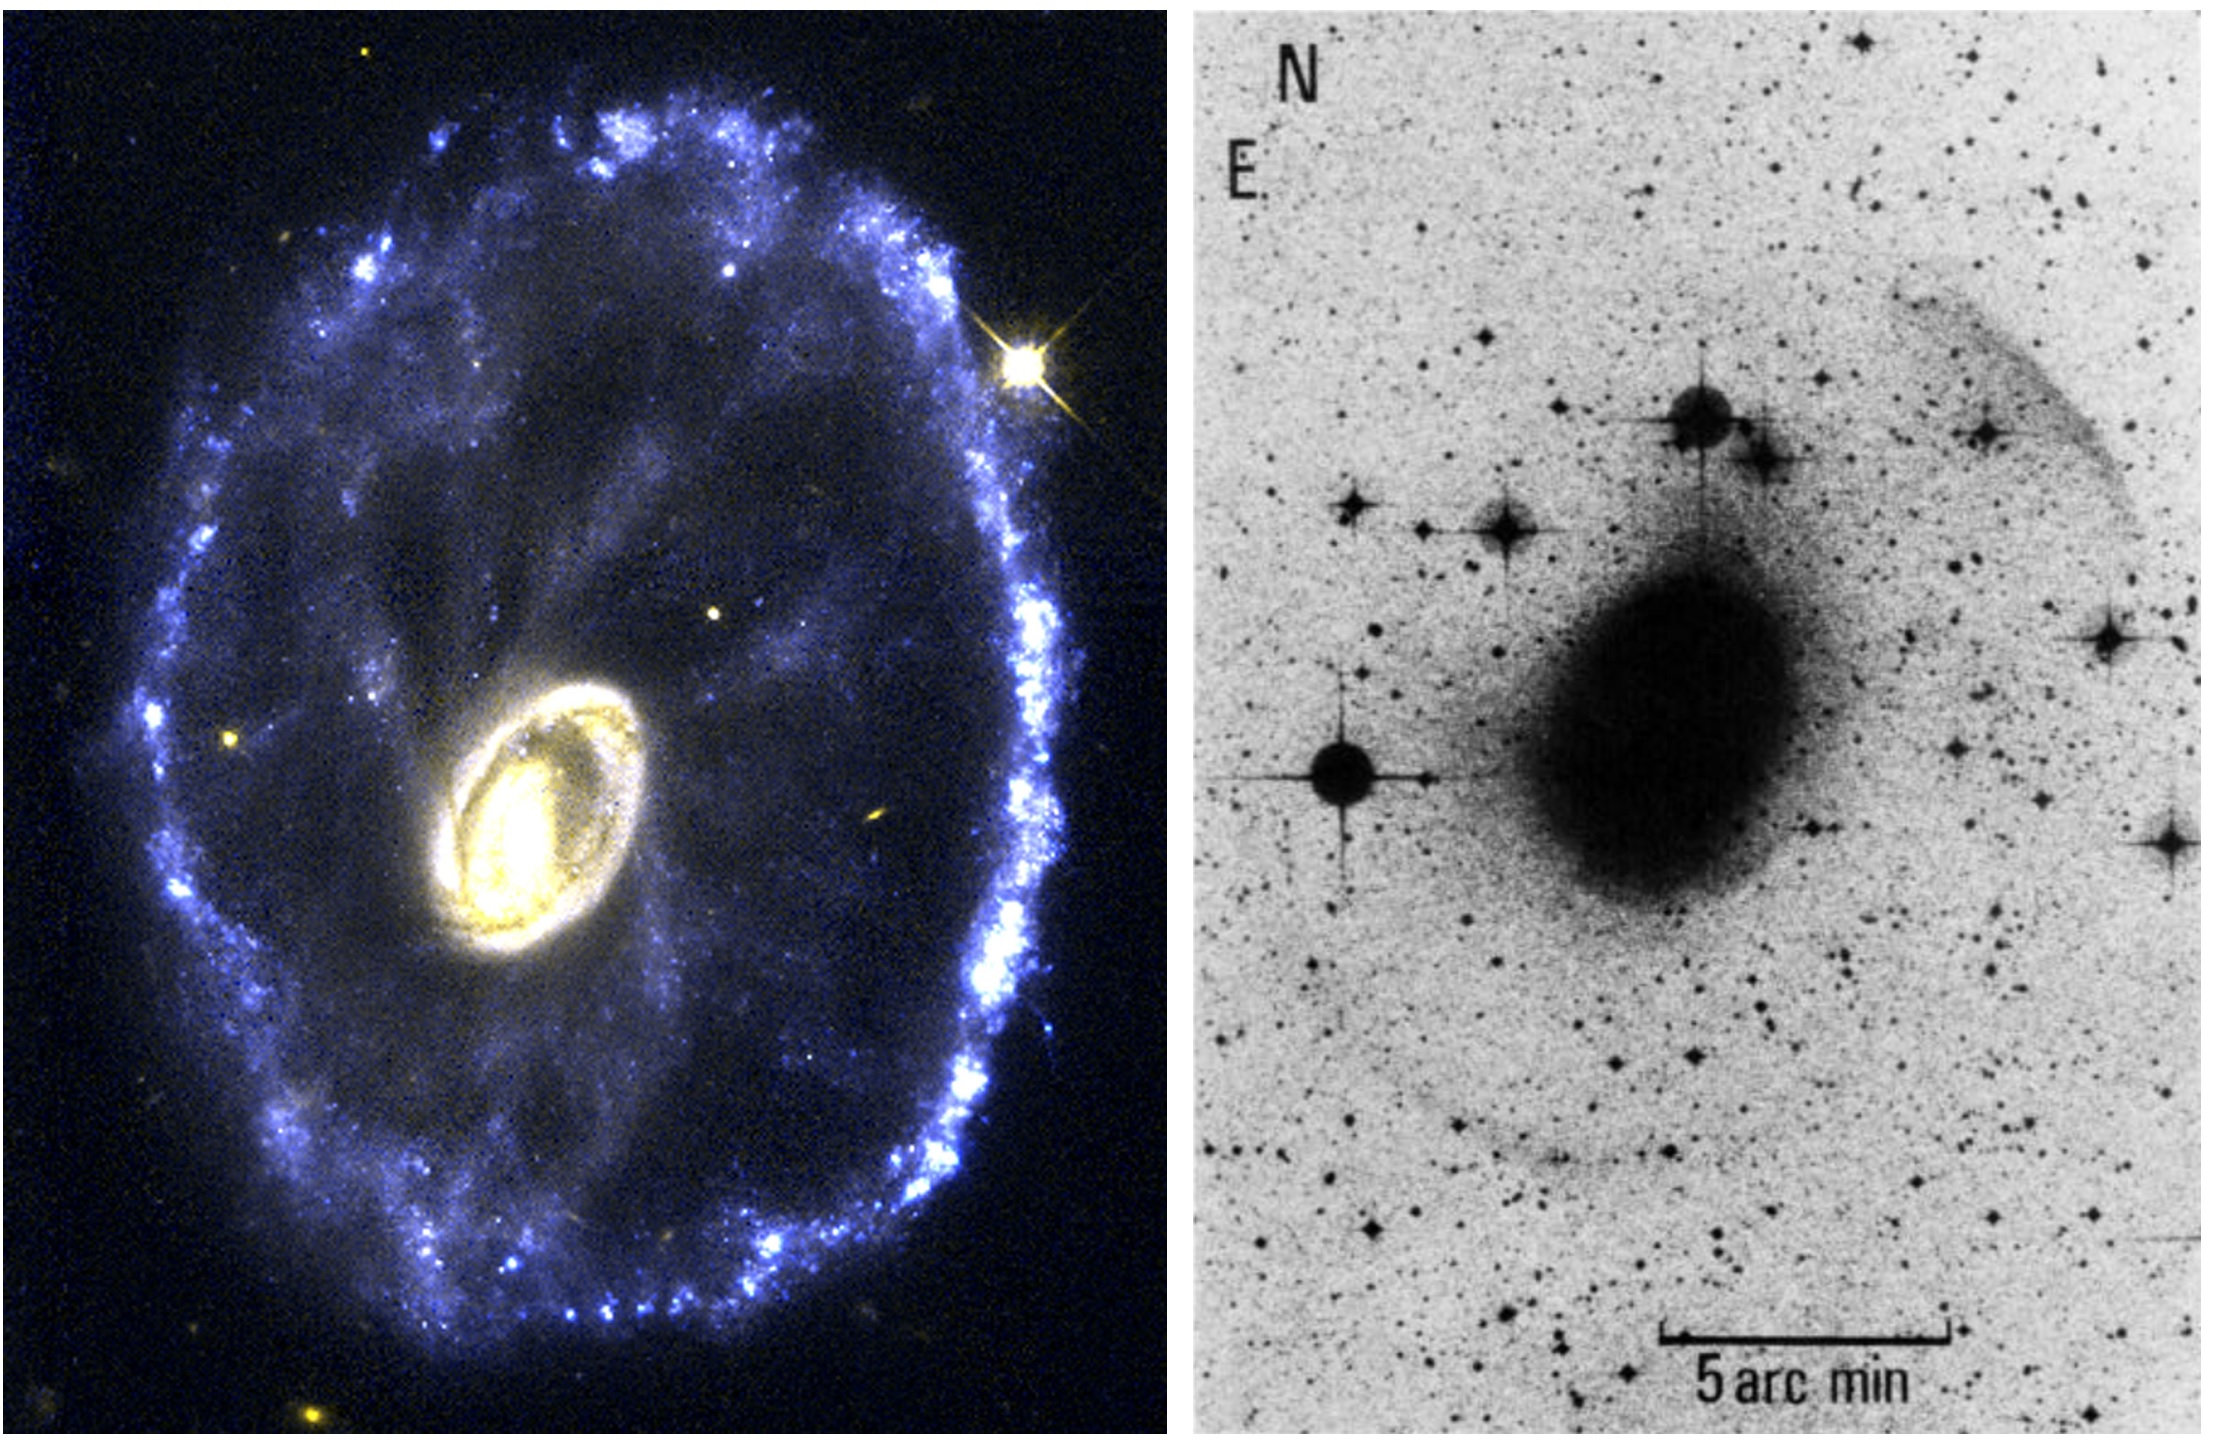
\includegraphics[width=0.95\textwidth]{Introduction/figures/shells-rings.jpg}
\caption[Examples of a collisional ring galaxy and a system containing shells.]{Examples of a collisional ring galaxy and a system containing shells. Left: The Cartwheel galaxy, the most famous ring galaxy to date. Ring galaxies can only be formed by a direct collision between two galaxies. The ring itself is composed of a region of the disk undergoing intense star formation due to the density wave passing through the disk from the impact of the secondary galaxy. Right: The system NGC 1344, showing two shells of stellar material surrounding it. This is formed by the condensation of stellar streams into clouds of stars. Cartwheel Galaxy Image: NASA / Hubble, NGC 1344 Image: \citet{1983ApJ...274..534M}}
\label{fig:tidal-features-ex}
\end{figure}

Finally, we find rings can form from galaxy interaction. These systems are often called ring galaxies or collisional ring galaxies. Figure \ref{fig:tidal-features-ex}\DIFdelbegin \DIFdel{s right }\DIFdelend \DIFaddbegin \DIFadd{'s left }\DIFaddend panel shows the Cartwheel Galaxy: a famous example of a ring galaxy. This ring is formed of young, hot stars and is formed only from the head-on collision with another system \citep{1976ApJ...209..382L}. The interaction to form this is so intense, that it causes a density wave to pass through the galactic disk which triggers intense star formation at its wake.

From the example of a ring galaxy, we see that interaction not only affects the stellar distribution of the galaxy, but also has direct impacts on the gas within it. As we have stated in previous sections, interaction and merging can induce enhancements in star formation and even lead to a starburst in a galaxy which brings about the complete quenching of the system.

\subsection{Star Formation Enhancement} 
\noindent As noted earlier, it is often observed in interacting and merging galaxies that the star formation is enhanced in some way. While to what level this enhancement is often debated between observations \citep{2003ApJ...582..668B, 2008MNRAS.385.1903L, 2011MNRAS.412..591P, 2022ApJS..261...34H} and simulations \citep{2007A&A...468...61D, 2008MNRAS.384..386C, 2013MNRAS.430.1901H, 2021MNRAS.503.3113M}, the underlying processes that lead to enhancement are well understood. First, by star formation enhancement we mean that the SFR either globally or in different regions of an interacting galaxy is higher when compared to isolated galaxies. Thus, some property of interaction is causing an increase in the star forming activity of the galaxies involved. 

The rate at which stars form is known to be directly related to the surface density of gas at any given piont within the galaxy, shown in equation \ref{eq:ks-law}. Due to an interaction the torques and gravitational forces upon the gas clouds \DIFaddbegin \DIFadd{leads to }\DIFaddend a loss of angular momentum. This causes the gas clouds to drift inwards, \DIFdelbegin \DIFdel{towards }\DIFdelend \DIFaddbegin \DIFadd{toward }\DIFaddend the galactic centre. As more gas clouds fall into the centre, the surface density of gas in this region increases. This in turn increases the SFR.

This is a simple explanation, and an easy idea to hold about driving the increase in star formation in interacting galaxies. As the morphology of the galaxy is compressed into a tidal feature, we see the same increase in the surface density of gas which leads to a further increase in the SFR. This movement and compression of gas into the galactic centre also has a secondary effect on the SMBH at the galactic centre. Increasing the gas density begins the feeding of the SMBH which causes the ignition of nuclear activity.

\subsection{Ignition of Active Galactic Nuclei}
\noindent The presence of an active galactic nuclei (AGN) in a galaxy is easy to identify observationally. When viewed them face on, the AGN is so luminous that it often outshines the entire bulge and disk of the galaxy. \DIFdelbegin \DIFdel{To study the galaxies they are present in }\DIFdelend \DIFaddbegin \DIFadd{The AGN dominates the SED of the galaxy, and }\DIFaddend we must carefully remove \DIFdelbegin \DIFdel{all contribution of the AGN to the underlying SED flux}\DIFdelend \DIFaddbegin \DIFadd{it using models to decouple the SED of the galaxy and the AGN}\DIFaddend . The bright flux we observe is from a long and complicated process of accretion of material onto the SMBH at the galactic centre \citep[for an excellent breakdown of the structure and evolution of AGN see][]{2012agn..book.....B}. The structure of material about the black hole is also complex, and results in many observational oddities. 

\DIFdelbegin \DIFdel{An }\DIFdelend \DIFaddbegin \DIFadd{Surrounding the black hole is an }\DIFaddend accretion disk of material\DIFdelbegin \DIFdel{that is orbiting the black hole structure exists}\DIFdelend . As this material accretes, it causes the SMBH to project powerful jets of radiation perpendicular to the accretion disk plane. These jets are highly luminous, and we observe them in the \DIFaddbegin \DIFadd{radio, }\DIFaddend optical, infrared and X-ray. Two populations of AGN have been discovered\DIFdelbegin \DIFdel{: }\DIFdelend \DIFaddbegin \DIFadd{, }\DIFaddend containing narrow and broad emission lines, named Seyfert 1 and Seyfert 2 AGN respectively. While at first thought to be two distinct types of AGN, these are believed to be one AGN population viewed from different angles \citep[for a review of the unification, see][]{2015ARA&A..53..365N}. This is possible as surrounding the accretion disk, there \DIFdelbegin \DIFdel{is a torus of material. This material is primarily dust, and highly absorbing of the }\DIFdelend \DIFaddbegin \DIFadd{are gas clouds which are either within or outside the nuclear region. Where these gas clouds are gives rise to the narrow and broad line emission observed in AGN spectra. 
}

\DIFadd{When we observe only narrow lines we are viewing the accretion disk through low density clouds. The gas of these clouds are photo-ionised by the continuum }\DIFaddend emission from the \DIFdelbegin \DIFdel{SMBH-accretion disk system. This means we only see }\DIFdelend \DIFaddbegin \DIFadd{central source itself. These are outside of the nuclear region and moving slowly (on the order a hundred km/s). The broad lines are observed when viewing the accretion disk through high density clouds which are located within the nuclear region close to the accretion disk. These clouds are moving fast (doppler broadening is observed to thousands of km/s). Putting this in the context of our AGN classifications, we only observe }\DIFaddend narrow line emission \DIFdelbegin \DIFdel{(}\DIFdelend \DIFaddbegin \DIFadd{in }\DIFaddend Seyfert 2 \DIFdelbegin \DIFdel{) when we observe the AGN through the torus and observing but observing both narrow and broad lines (Seyfert }\DIFdelend \DIFaddbegin \DIFadd{AGN, so we are observing the nuclear region through low density, slow moving gas clouds out. When we observe Seyfert }\DIFaddend 1 \DIFdelbegin \DIFdel{) of emission when not viewed through the torus. }\DIFdelend \DIFaddbegin \DIFadd{galaxies, we are viewing the nuclear region through dense gas clouds which lie close to the central engine. This entire system is encased in a dusty torus of material. We cannot observe the nuclear region through this torus, thus, hiding emission lines from our observations at perpendicular viewing angles.
}

\DIFadd{There are many other categories of AGN beyond Seyfert 1 and 2's. }\DIFaddend As we move to higher luminosities, we get further populations of AGN such as blazars, quasars, radio-quiet and radio-loud systems. These classifications are all dependent upon the inclination at which we are viewing the AGN system and the material in the line of sight.

From this description of an AGN structure we can see how galaxy interaction increases the likelihood of nuclear ignition. AGN require large volumes of gas and dust to be present at the galactic core\DIFdelbegin \DIFdel{; }\DIFdelend \DIFaddbegin \DIFadd{, }\DIFaddend a surge of which is caused by interaction \citep[][provides an excellent summary of this process from the point of view of simulations]{2008ApJS..175..356H}. However, what is often surprising from observations of samples of interacting systems is the meagre increase in the AGN fraction within them. There have been many \DIFdelbegin \DIFdel{hypothesis }\DIFdelend \DIFaddbegin \DIFadd{hypotheses }\DIFaddend as to why this might be, from a delay in the AGN ignition \citep{2011MNRAS.418.2043E} to AGN flickering \citep{2015MNRAS.451.2517S}. A delay in AGN ignition would make sense, again, in the context of the structure we have just discussed. As gas and dust are moved into the galactic core, they do not necessarily immediately move directly around the SMBH and may take time to get there. There may be other mechanisms at work within the AGN itself that causes suppression of ignition for some time. This could also produce the AGN flickering, where material may be periodically \DIFdelbegin \DIFdel{cutoff }\DIFdelend \DIFaddbegin \DIFadd{cut off }\DIFaddend from the SMBH.

It cannot be disputed that the sudden movement of gas into the galactic centre during interaction appears like an obvious way for AGN activation to occur. However, this movement of gas around the galaxy and use in star formation and use or ejection \DIFdelbegin \DIFdel{in }\DIFdelend \DIFaddbegin \DIFadd{by }\DIFaddend an AGN can start the quenching of the galaxy. 

\subsection{Quenching of Galactic Systems}
\noindent During the interaction of two galaxies there is significant movement of gas, AGN activation and large increases in star formation across the galaxy. However, a galaxy only has a limited reservoir of gas available to it. Therefore, this sudden increase in gas usage in multiple different processes leads to the gas being used in a shorter timescale than expected. Once the gas is used, and the gas density drops significantly, star formation and AGN will rapidly cease and the colour of the galaxy \DIFaddbegin \DIFadd{will change to red}\DIFaddend . This process is called quenching.

This rapid quenching of systems is different to what is expected \DIFdelbegin \DIFdel{in the field}\DIFdelend \DIFaddbegin \DIFadd{for isolated galaxies}\DIFaddend . Galaxies gradually use their gas over long periods of time forming stars and slowly quench as the average gas density across the disk reduces to the point of very low SFRs \citep{2010ApJ...721..193P} in `mass quenching'. A system can also be quenched by the environment in `environment quenching'. However, by concentrating gas and increasing the gas density in an interaction, even if a galaxy had previously stopped forming stars it is able to commence star formation again and use the remaining gas entirely. Thus, we often seen increases in the SFR during and immediately after an interaction but then the sudden shut off of SFR shortly after it \citep{2022MNRAS.517L..92E}. 

The \DIFdelbegin \DIFdel{sudden use of }\DIFdelend gas is not \DIFdelbegin \DIFdel{just from it being }\DIFdelend \DIFaddbegin \DIFadd{only }\DIFaddend used in star formation, but also from stellar feedback around the areas where the stars are forming. As these new stellar populations form OB-type stars very quickly die and cause an increase in the rate of supernova. This, in turn, creates strong shocks and winds that drive the molecular gas out of the galaxy at very high speed \citep{2013Natur.499..450B, 2018ApJ...864L...1G}. A similar process can occur due to the AGN in the galaxy. These objects drive strong winds across the galactic system. These winds can also act to drive out gas \citep{2014A&A...562A..21C, 2016Natur.533..504C, 2018MNRAS.480.3993B} and cause the cessation of star formation.

\section{Identifying Interacting and Merging Galaxies}
\noindent We have described and explored the effects of interaction and merging across the galaxy population. We have described the basic properties of galaxies and how these are differ when compared to interacting galaxies. However, we are only able to fully understand these differences by using samples of interacting galaxies and comparing them to control samples.

% This section is going to be re-written as I talk at length about these catalogues in the next section.
The first samples of interacting galaxies were identified by eye. The earliest interacting galaxy catalogue was the \citet{1966ApJS...14....1A} Atlas of Peculiar Galaxies. This contained 166 interacting systems. This was quickly added to with a 2-part edition of the \citet{1977A&AS...28....1V} catalogue, providing a further 268 systems to the original \citet{1966ApJS...14....1A} catalogue. Both of these catalogues contained major interactions, where clear tidal features easily put them into the interacting galaxy classification. These samples were also not large enough to make statistical, representative statements about the interacting galaxy population. Thus, larger catalogues had to be created.

Later catalogues often used visual classification to find interacting and merging galaxies. A very successful example is from the Galaxy Zoo collaboration which created a catalogue of 3,003 interacting galaxies identified by citizen scientists based on morphology \citep{2010MNRAS.401.1043D}. However, a limitation was found when visually classifying interacting galaxies. With no information on the redshift, and therefore of 3D distribution of a galaxy pair, it is very difficult to distinguish `close pairs' from truly interacting pairs. A close pair, in this context, is two galaxies which appear to be very close together in the sky in the 2D projection of the sky but are actually at different redshifts. This means they are not actually close together in 3D space and cannot be interacting. Many interacting galaxy samples created by visual classification must discard large numbers of false positives from their sample \citep{2020MNRAS.492.2075B, 2022A&A...661A..52P}. As machine learning algorithms started to be used in galaxy classification, this problem of contamination by close pairs continued.

Neural networks play an increasingly central role in galaxy classification. As the size of observational samples has increased (e.g. RC3, with $\sim 20,000$ galaxies, \citealt{1991rc3..book.....D}; 2dF, with $\sim 200,000$ galaxies \citealt{2001MNRAS.328.1039C}; SDSS, $\sim 1,000,000$ galaxies with spectra, \citealt{2000AJ....120.1579Y, 2009ApJS..182..543A}; Legacy Survey of Space and Time, with $\sim 20,000,000,000$ galaxies expected, \citealt{2019ApJ...873..111I}), so has the challenge of visually classifying each galaxy individually. Rather, a neural network can now be trained to make morphology classifications of galaxies using a much smaller subset of visually classified galaxies.
\DIFaddbegin 

\DIFaddend A neural network is a layered structure of interconnected nodes which can pass information to one another. Each node has a weight assigned to it which allows it to alter the input and then pass on the weighted output. If the weighted output is above or below some value, the output is set zero. The input in this context can be some information about a galaxy, a section of an image or an underlying parameter estimation. These nodes all interconnect through many different layers where they all perform operations on their input and provide weighted outputs. The weighted outputs from the final layer are then passed to a classification layer which outputs either a formal classification or some value that can be mapped to a classification by a user.

A formal classification can be made in this way by training the neural network to recognise certain features of an image. Training a neural network in supervised learning involves providing it with a training set of fully annotated data so it can `learn' classifications. \DIFaddbegin \DIFadd{If the training set is sufficiently large, it is split into batches that the neural network will iterate over. }\DIFaddend To train, the neural network \DIFdelbegin \DIFdel{iterates through the provided }\DIFdelend \DIFaddbegin \DIFadd{is fed each batch of the }\DIFaddend training set and makes classifications upon each \DIFdelbegin \DIFdel{input. It then checks how many it got right and how many wrong, and then tweaks the weights of each node. It then makes the classifications again and checks whether it got more right or wrong. This is done }\DIFdelend \DIFaddbegin \DIFadd{item within them. It iterates through each batch until it has made classifications on the entire training set. A loss function is then used to measure how accurate the model was based on how many classifications were correct and incorrect. The weights of the model are then updated by back propagating through model. Once this is completed, an epoch of the training has been completed. This process is repeated }\DIFaddend through many epochs \DIFdelbegin \DIFdel{of the training set, it gradually tweaks its internal weights such that it }\DIFdelend \DIFaddbegin \DIFadd{with model weights being tweaked each time and the a loss function being minimised in some way. Once this has been achieved, the model }\DIFaddend should be able to make \DIFdelbegin \DIFdel{the same }\DIFdelend classifications on an unknown dataset and \DIFdelbegin \DIFdel{recognise images with similar classifications }\DIFdelend \DIFaddbegin \DIFadd{make accurate classifications on data similar }\DIFaddend to the training set. Thus, it is important that the training set is large and is representative of the full \DIFdelbegin \DIFdel{parameters }\DIFdelend \DIFaddbegin \DIFadd{parameter }\DIFaddend space a user wishes to classify.

In morphology classification, the workhorse neural network is the convolutional neural network \citep[CNN; examples include][]{2010MNRAS.406..342B, 2015ApJS..221....8H, 2020MNRAS.491.1554W, 2023ApJ...944..124T}. A CNN takes an image and breaks it down into smaller subsections in a \DIFdelbegin \DIFdel{convolutional layer. These smaller subsections - essentially arrays of different sections of }\DIFdelend \DIFaddbegin \DIFadd{its convolutional layers. These are the layers immediately after the input layer, and reduce the dimensions of the image by applying a convolutional filter of a specified size to the image. This, essentially, conducts the dot product between a group of the pixels in the image and }\DIFaddend the \DIFdelbegin \DIFdel{image }\DIFdelend \DIFaddbegin \DIFadd{filter. This returns a single integer which represents a group of pixels in the image. This integer is then passed to the next layer of the CNN. This is done across the entire image, and has the effect of reducing the dimensionality of the image by a factor of the size of the convolutional filter. There is then a ReLU activation immediately after this which makes all negative integers equal to zero. After the convolutional layer, there is a pooling layer. This layer dramatically reduces the dimensionality of the output of the convolutional layer by pooling it by a specified filter and dimension.
}

\DIFadd{This can be repeated many times, depending on the dimensions of the image. The aim is reduce the dimensionality of the image as much as possible for passing to the fully connected layers while maintaining the representation of the image as best as possible. These representations }\DIFaddend - \DIFdelbegin \DIFdel{are passed through the neural network operations and activations and are altered by the weights at each node. Depending on the number of layers in the CNN, the image may be sub-divided, convolved and weighted many timesbefore being fed into }\DIFdelend \DIFaddbegin \DIFadd{essentially integers representing different sections of the image - are passed through the neural network operations as described previously. The output features from the fully connected layer then go to }\DIFaddend a classification layer\DIFdelbegin \DIFdel{which outputs the final classification . The real }\DIFdelend \DIFaddbegin \DIFadd{, often a }\texttt{\DIFadd{Softmax}} \DIFadd{or }\texttt{\DIFadd{Logistic}} \DIFadd{layer, which returns the classification to be interpreted. The }\DIFaddend power of a CNN such as described is that it is able to recognise features in an images. For instance, tidal features, AGN or the whole morphology of the galaxy such as ellipticals or disks \citep[e.g][]{2018MNRAS.479..415A,2020ApJ...895..112G, 2022MNRAS.511.3330T, 2023ApJ...944..124T}. 

However, using a CNN for the purposes of identifying interacting galaxies still introduces the same problems as using visual identification. While the classifications it makes on the morphology of interacting galaxies, or on two galaxies being near each other in an image, it faces the same contamination from close pairs.

New methods combining CNNs with morphological parameterisations of a galaxy are being developed to overcome this issue. This has found some success in correctly identifying interacting galaxies fom morphology alone \citep{2023ApJ...958...96R}. Other works have turned to training CNNs on simulated data\DIFdelbegin \DIFdel{; }\DIFdelend \DIFaddbegin \DIFadd{, }\DIFaddend where the training set could be controlled and large enough to span the entire parameter space of interaction. These training sets would also have the advantage of being completely free of contamination. However, when applied to observational data it was found that the accuracy of such models \DIFdelbegin \DIFdel{completely }\DIFdelend breaks down \citep{2019MNRAS.490.5390B, 2020A&C....3200390C}. Thus, creating large and pure interacting galaxy samples remains a task to complete, and the method being it an open question.

\DIFaddbegin \DIFadd{Using morphology, and the existence of tidal features, is not uniform across redshift however. As galaxies are observed at higher redshifts they are found to have both dimmer surface brightnesses and, often, to have a smaller angular size. This is not due to evolutionary effects, but from cosmological effects and has direct consequences on our classification methods of interacting galaxies. We will lose sensitivity to detecting tidal features about interacting and merging galaxies as their redshift increases and our samples will be biased toward those systems with high surface brightnesses.
}

\section{\DIFadd{Cosmological Effects}}
\noindent \DIFadd{Another fundamental obstacle to successfully identifying interacting and merging galaxies are two cosmological effects: surface brightness dimming of a galaxy and the changing angular size of a galaxy. Both of these are a result of the Universe expanding. For instance, we would expect that the luminosity per unit area of a galaxy would remain constant if the Universe was static. However, because the Universe is expanding three things are changing when we observe a galaxy: the photons arrive at a different rate, the wavelengths of the photon changes and the angular size of the galaxy changes (gets smaller) with time.
}

\DIFadd{The surface brightness is defined as the luminosity within some defined area, in this case angular size on the sky. So, because the angular size is changing while the luminosity remains the same, the surface brightness is decreasing. This relation between the surface brightness and redshift was originally derived using this approach by \mbox{%DIFAUXCMD
\citet{1930PNAS...16..511T, 1934rtc..book.....T}}\hspace{0pt}%DIFAUXCMD
. If we have a galaxy at some redshift, $z$, its surface brightness will be dimmed by
}\begin{equation}\DIFadd{\label{surf_dimming}
I_{0} = \frac{I_{e}}{(1+z)^{4}}.
}\end{equation}
\DIFadd{Here, $I_{0}$ is the observed surface brightness of an object and $I_{e}$ is its intrinsic surface brightness. Due to this, a galaxy observed at z = 1 will be 16 times dimmer than the same galaxy observed in the local Universe ($z\sim0$). 
}

\DIFadd{We use the detection of tidal features to classify interacting and merging systems. These features often lie in the low surface brightness regime. Therefore, even in the local Universe, we are observing them at the very limiting magnitudes of many of our telescopes. So, when attempting to make classifications at high redshifts andwhere surface brightness dimming begins to take an effect, we will lose the ability to detect the tidal features of an interacting galaxy. Therefore, we risk being biased only those galaxies with a surface brightness \mbox{%DIFAUXCMD
\citep{2014ApJ...796..102C}}\hspace{0pt}%DIFAUXCMD
, or mis-representing the underlying structure of a galaxy entirely \mbox{%DIFAUXCMD
\citep{2018MNRAS.473.2701D}}\hspace{0pt}%DIFAUXCMD
.
}

\DIFaddend \section{This Thesis}
% Potentially expand this or change the title.
\noindent The primary focus of this thesis is investigating and constraining the relationship between galaxy interaction and evolution. The list of unresolved questions about galaxy interaction is long and complex, but we will focus on the following questions here:

\begin{itemize}
\item What is the relation between galaxy interaction and the enhancement in star formation?
\item What is the relation between galaxy interaction and the fraction of AGN?
\item At what point in an interaction do we find \DIFdelbegin \DIFdel{these relations are greater than }\DIFdelend \DIFaddbegin \DIFadd{enhancement in star formation and a change in fraction of AGN }\DIFaddend compared to non-interacting galaxies?
\item What is the conclusive relationship between the dynamical timescale of interaction, the formation of tidal features and the above effects?
\end{itemize}

To fully answer these questions three components are required: first, a large statistically significant sample of interacting galaxies; second, available ancillary data of these systems to make inferences between the underlying processes in interaction and their parameters; and thirdly, the tools \DIFaddbegin \DIFadd{to }\DIFaddend constrain the dynamical timescales of each system. This thesis details methodologies which \DIFdelbegin \DIFdel{acheive }\DIFdelend \DIFaddbegin \DIFadd{achieve }\DIFaddend these goals. First, in Chapter \ref{chapter2}, we create the largest interacting galaxy catalogue to date through combining morphological classification with novel methods of machine learning, data extraction and analysis. We then use this catalogue, in Chapter \ref{chapter3}, by matching to existing ancillary catalogues and conduct our own inferences about the relationship between galactic parameters and underlying processes. However, we find that we can only constrain this relationship to a very general point. We require tighter constraints on the dynamical timescale of the interactions in our sample to further explore the relationship between galaxy evolution and interaction. In Chapter \ref{chapter4}, we describe software we have built that will conduct such constraint in the context of Bayesian statistics and galactic parameterisation. We will describe the results we have found by applying it to a small, well constrained, interacting galaxy sample and then describe the limitations of the approach in terms of computational efficiency. Finally, in Chapter \ref{chapter:conclusion} we summarise our results, describe them in the context of current works and speculate about the future work to advance them.

Where necessary, we use a Flat $\Lambda$CDM cosmology with $H_{0} = 70\mathrm{kms}^{-1}\mathrm{Mpc}^{-1}$ and $\Omega_{M} = 0.3$. Hereafter in this thesis, when referring to an interacting galaxy we are referring to a galaxy which has undergone one or multiple flybys by a secondary galaxy and caused a tidal disturbance. A merging galaxy is the final state of these flybys, where two or more systems have coalesced to form a highly morphologically irregular system.
